\documentclass[12pt,a4paper]{article}
\usepackage[utf8]{inputenc}
\usepackage[spanish]{babel}
\usepackage{amsmath}
\usepackage{amsfonts}
\usepackage{amssymb}
\usepackage{makeidx}
\usepackage{graphicx}
\usepackage[left=2cm,right=2cm,top=2cm,bottom=2cm]{geometry}
\author{Felipe Alvarado Galicia}
\title{PAR DE ROTACIÓN Y CUATERNIOS}
\date{Materia: Cinematica de Robots\\
17 de septiembre de 2019}

\begin{document}
\maketitle 
\includegraphics[scale=1]{logo1.png}\\
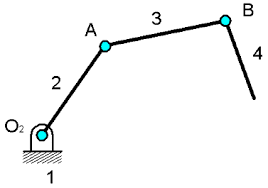
\includegraphics[scale=1]{imag5.png} 
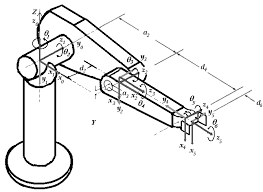
\includegraphics[scale=1]{imag8.png}\\\\\\\\\\\\\\\\\\\\\\\\\\\\\\\\\\\\\\\\\\\\\\

\section{Par de rotación}
EL PAR DE ROTACIÓN\\
El cálculo del par es necesario para asegurar la rotación del conjunto que tiene en cuenta:\\
   • las cargas en la maquina\\
   • las masas de arrastre\\
   • las distancias de estas masas respecto al eje de rotación\\
   • las velocidades y las aceleraciones\\
   • las pares resistentes\\

Dos tipos de par son diferenciados:\\
   El par de giro a la puesta en marcha : Cd=Crv+Crc\\
   El par de giro a la aceleración: Cg=Crv+Crc+Ca\\

Crv = Par resistente del rodamiento vacío\\
Crc = Par de rotación debido a las cargas\\
Ca = Par de rotación\\
Cd = Par de puesta en marcha\\
Todos estos pares estan expresados en kNm\\
Crc : PAR DE ROTACION DEBIDO A LAS CARGAS\\
El par necesario a la puesta en maarcha de la rotacion tiene en cuenta las cargas en la corona y de los rozamientos de los componentes.\\
Coronas con bolas :\\
Crc = [ (13,11 MT / Ø m ) + 3 FA + 11,34 FR ] Ø m . 10 -3\\\\
Coronas con rodillos:
Crc = [ ( 15,3 MT / Ø m ) + 3,75 FA + 8,19 FR ] Ø m . 10 -3\\\\
MT = Momento resultante en kNm\\
Ø m = Ø medio de rodamiento en mt\\
FA = carga axial en  kN\\
FR = carga radial en kN\\\\
Ca : PAR DE ACELERACION\\
 El par necesario para pasar las cargas de velocidad inicial a la velocidad final durante el timepo es definido por :\\
Ca = [ ( 3.1416 . n . l ) / 30 . t ] . 10-3\\\\
t = Tiempo de aceleracion en segundos.\\
n = Variacion de velocidad en revoluciones / min (Velocidad final- Velocidad inicial)\\
l = Momiento de inercia de la maquinas en Kg . m*m\\
l = l1 + l2 + l3 + ..... ln\\\\
donde l1 à ln = momiento de inercia de las masas en movimiento respecto a eje de rotación expresado en Kg . m*m\\\\
En general, tenemos :\\
l1 = G1 * r1*rl\\
ln = Gn * rn*rn\\
G1 à Gn = Masas de los diferentes elementos en rotacion expresados en Kg.\\
r1 à rn = Distancias entre el centro de gravedad de las masas y del eje de rotacion de la corona expresada en metros.\\\\
\section{Cuaternios}
Los cuaterniones unitarios proporcionan una notación matemática para representar las orientaciones y las rotaciones de objetos en tres dimensiones. Comparados con los ángulos de Euler, son más simples de componer y evitan el problema del bloqueo del cardán. Comparados con las matrices de rotación, son más eficientes y más estables numéricamente. Los cuarteniones son útiles en aplicaciones de gráficos por computadora, robótica, navegación y mecánica orbital de satélites.\\
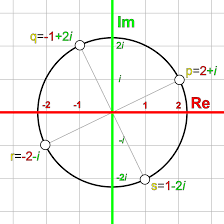
\includegraphics[scale=1]{imag6.png}\\
Entonces un cuaternión es un número de la forma a + bi + cj + dk, donde a, b, c, y d son números reales unívocamente determinados por cada cuaternión.\\

La multiplicación de los cuaterniones no es conmutativa: ij = k, ji = -k, jk = i, kj = -i, ki = j, ik = -j. Los cuaterniones son un ejemplo de cuerpo asimétrico, una estructura algebráica parecida a un cuerpo pero no conmutativo en la multimplicación. La multplicación es asociativa y todo cuaternión no nulo posee un único inverso. Forman un álgebra asociativa cuadridimensional sobre los reales y los complejos forman un subconjunto de ella, los cuaterniones no forman un álgebra asociativa sobre los complejos.\\
El valor absoluto de un cuaternión z = a + bi + cj + dk queda definido por |z|2 = a2 + b2 + c2 + d2.\\
Usando la función distancia definida como d(z,w) = |z - w|, los cuaterniones forman un espacio métrico y todas las operaciones aritméticas son continuas.\\
También tenemos que |zw| = |z| |w| para cualesquiera cuaterniones z y w.\\
Usando como norma el valor absoluto, los cuateriones conforman un álgebra de Banach real.\\
El conjunto de los cuaterniones de valor absoluto 1 forman una esfera tridimensional S3 y un grupo (incluso grupo de Lie) con la multiplicación. Este grupo actúa, mediante conjugación, sobre la copia de R3 constituida por los cuaterniones cuya parte real es cero. No es difícil comprobar que la conjugación por un cuaternión unidad de parte real cos t es una rotación de ángulo 2t con el eje de giro en la dirección de la parte imaginaria. Así, S3 constituye un recubrimiento doble del grupo SO(3) de matrices ortogonales 3x3 de determinante 1; es isomorfo a SU(2), el grupo de matrices 2x2 complejas unitarias y de determinante unidad.\\
Para más detalles sobre la rotación en el espacio mediante los cuaterniones, véase cuaterniones y rotación en el espacio.\\
Sea A el conjunto de cuaterniones de la forma a + bi + cj + dk donde a, b, c y d son, o todos enteros o todos racionales con numerador impar y denominador 2. El conjunto A es un anillo y un retículo. Hay 24 cuaterniones unitarios en este anillo y son los vértices de un politopo regular, llamado {3,4,3} en la notación de Schlafli.\\
Los cuaterniones se utilizan a menudo en gráficos por computadora (y en el análisis geométrico asociado) para representar la orientación de un objeto en un espacio tridimensional. Las ventajas son: conforman una representación no singular (comparada con, por ejemplo, los ángulos de Euler), más compacta y más rápida que las matrices.\\

\end{document}